% !TeX spellcheck = en_GB

%%%%%%%%%%%%%%%%%%%%%%%%%%%%%%%%%%%%%%%%%%%%%%%%%%%%%%%%%%%%%%%%%%%%%%%%
\chapter{Related Work}
\label{sec:relatedWork}

This chapter discusses relevant work for the ChaCha plug-in implementation and was therefore reviewed during the work on this thesis.

%%%%%%%%%%%%%%%%%%%%%%%%%%%%%%%%%%%%%%%%%%%%%%%%%%%%%%%%%%%%%%%%%%%%%%%%
\section{Salsa20 Cipher Family}
\label{sec:salsaCipher}

The ChaCha cipher family is based on the 256-bit stream cipher family Salsa20.
\noindent
Salsa20/20, the 20 rounds variant, was developed by Daniel J. Bernstein in 2005 \cite{salsaspec} and submitted to eSTREAM, a European project to ``to promote the design of efficient and compact stream ciphers suitable for widespread adoption'' \cite{estream}.

It uses only add-rotate-XOR (ARX) operations for encryption which prevents timing attacks since they run in constant time on basically all platforms. Beside 256-bit keys, it also supports 128-bit keys. It internally uses a hash function which transforms a 512-bit state, consisting of the key, four 32-bit constants, a 64-bit initialization vector and a 64-bit counter, into a keystream block. For following keystream blocks, only the counter is incremented in the initial state before applying the hash function. This means that Salsa20 shares the same implementation advantages as block ciphers in counter mode, in particular the ability to generate output blocks in any order and in parallel \cite{salsaspec}.

Bernstein later introduced other variants with 8 and 12 rounds, named Salsa20/8 and Salsa20/12, to let users decide for a faster, but less secure cipher. Other round variants like 9, 10 or 11 were not introduced because the difference in speed would be insignificant \cite{salsa812}. The ChaCha cipher family received the same round variants. 

There is also a variant of Salsa20 called XSalsa20 which supports 192-bit initialization vectors. Since its implementation varies quite a bit from the Salsa20/r variants and Bernstein introduced XSalsa20 as part of a new cipher family (based on Salsa20), this cipher is of no relevance for this thesis \cite{xsalsa20spec}. There is a XChaCha20 variant but it ``is currently not widely implemented outside the libsodium library [a software library for cryptography], due to the absence of formal specification'' \cite{xchacha20}.

The specification of Salsa20 is very relevant for ChaCha because the specification for ChaCha only mentions the differences \cite{chachaspec}. Therefore, to implement ChaCha, one has to also read through the specification of Salsa20.  However, Chapter \ref{chap:chacha} will summarize the specification of ChaCha without assuming prior knowledge about Salsa20.

%%%%%%%%%%%%%%%%%%%%%%%%%%%%%%%%%%%%%%%%%%%%%%%%%%%%%%%%%%%%%%%%%%%%%%%%

\section{Salsa20 CrypTool 2 Plug-in}
\label{sec:salsaCT2Plugin}

\begin{figure}
\centering
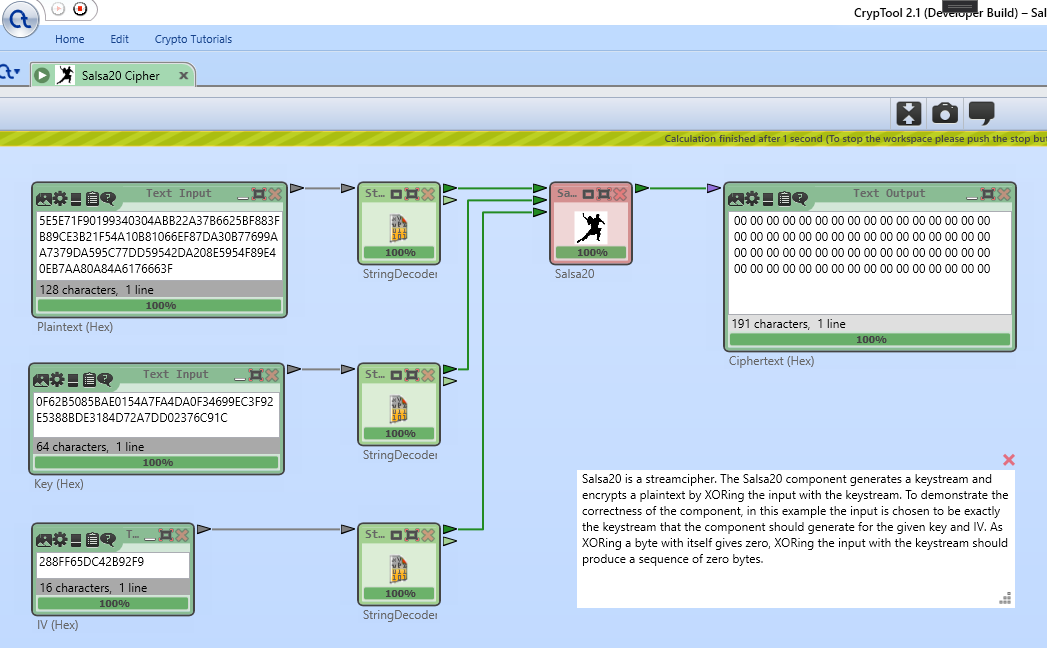
\includegraphics[width=\textwidth]{figures/ct2/salsa-crop.png}
\caption[Salsa20 CT2 template]{CT2 template for the already existing Salsa20 plug-in}
\label{fig:salsa.template}
\end{figure}

CrypTool 2 already has a plug-in for the Salsa20 cipher but without a visualization. Figure \ref{fig:salsa.template} shows the CT2 template for the plug-in. Templates are prepared workspaces for a plug-in where all necessary components to run the plug-in are already included and properly connected.

During the work on the ChaCha visualization, we discussed if the code could be reused to create a visualization for the Salsa20 cipher family. However, this would at least need adaption of the XAML code since the state is built up differently. Also the quarter-round function is slightly different which also needs to be reflected in the visualization.

Nonetheless, it should be possible to reuse most of the codebase used for the ChaCha visualization, especially the underlying navigation system and the storage and retrieval mechanism for the intermediate results. This will further be discussed in Chapter \ref{sec:futureWork}.

%%%%%%%%%%%%%%%%%%%%%%%%%%%%%%%%%%%%%%%%%%%%%%%%%%%%%%%%%%%%%%%%%%%%%%%%
\section{Other CrypTool 2 Cipher Visualizations}
\label{sec:otherCT2CipherVisualizations}

This section is all about other existing CT2 cipher visualizations and which ideas originated from them. The plug-ins were also created by students during their bachelor's thesis.

\subsection{AES Visualization}
\label{sec:aesVisualization}

Matthias Becher created a visualization for the AES cipher during his bachelor's thesis in 2016. It was the visualization of which the most inspiration was taken from for the ChaCha visualization. Reading through his bachelor's thesis was very useful since he encountered similar problems. For example, he wrote the following in his bachelor's thesis:

``The first big decision that had to be made was whether the states after each encryption operation would be calculated during the visualization or precalculated and stored at the start of the execution. One feature the plug-in should have was to not only jump ahead to later operations but also to go back to previous ones. That means if the values were calculated during the visualization every time you went back they would have to be recalculated from the start. Therefore, I decided to precompute and store results of each operation in an array of byte arrays..'' \cite{aesthesis}

We came to the exact same conclusion that the values need to be precalculated for the reasons he mentioned.

\begin{figure}
\centering
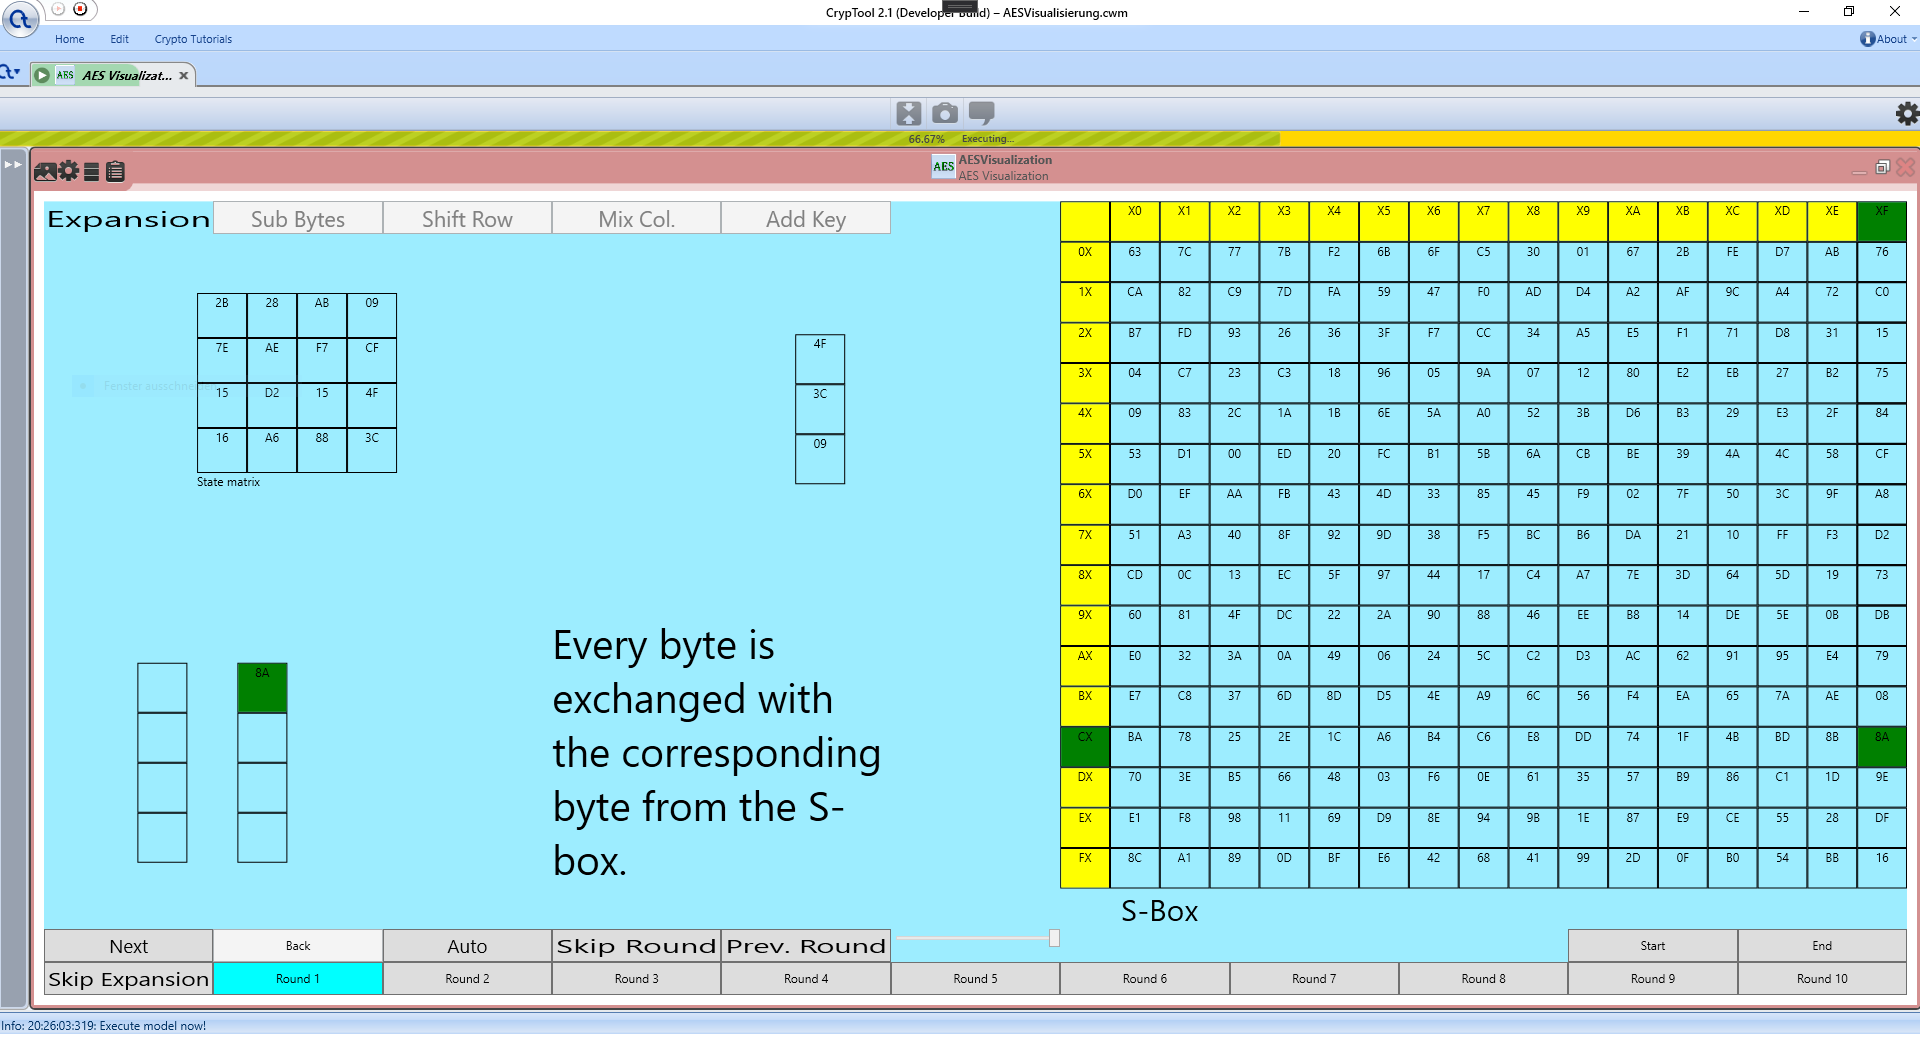
\includegraphics[width=\textwidth]{figures/ct2/aes.png}
\caption{AES visualization plug-in}
\label{fig:aes}
\end{figure}

Looking through his visualization, his usage of background coloring was very useful to catch the user's attention. This is shown in Figure \ref{fig:aes}. Therefore, there is a similar mechanic during the ChaCha hash function visualization where a light blue background is put onto the state elements which are used as the quarter-round input. Also during the quarter-round execution, background coloring is extensively used to indicate where the user should pay attention.

Another thing adopted from his visualization was the navigation in the top-left corner where the page navigation for the ChaCha visualization is placed. \\
What is different regarding navigation is to not show so many buttons all the time to the user. It was quite overwhelming to see all the buttons in the bottom navigation bar on the start even though they were disabled. Therefore, on pages which have no actions, there are no buttons in the bottom row. For the ChaCha hash function, which needed more detailed navigation, the navigation bar looks similar expect that it uses arrow buttons and text inputs instead of buttons for every single round. This decreased the amount of buttons while maintaining a similar degree of navigation.

Further, it was confusing that the ``Back'' button during the ``Expansion'' or ``Encryption'' step was disabled. For the ChaCha plug-in, the user should be able to navigate to any step in the visualization fairly simple. To achieve this, the page navigation in the top-left corner stays the same on every page and tells the user on which page he currently is with bold font. This means the user knows that if he wants to go to a different page, he needs to select the page there. Additionally, every single action on each page is numbered together with an action text input and how many actions a page has in total. The text input makes it possible for the user to immediately jump to an action. If he does not know the number of the action he wants to go, there are also buttons labeled with descriptive names on the pages with actions. For example, the page about the state setup has buttons to immediately go to the start or end of the key encoding step.

\subsection{DES Visualization}
\label{sec:desVisualization}

\begin{figure}
\centering
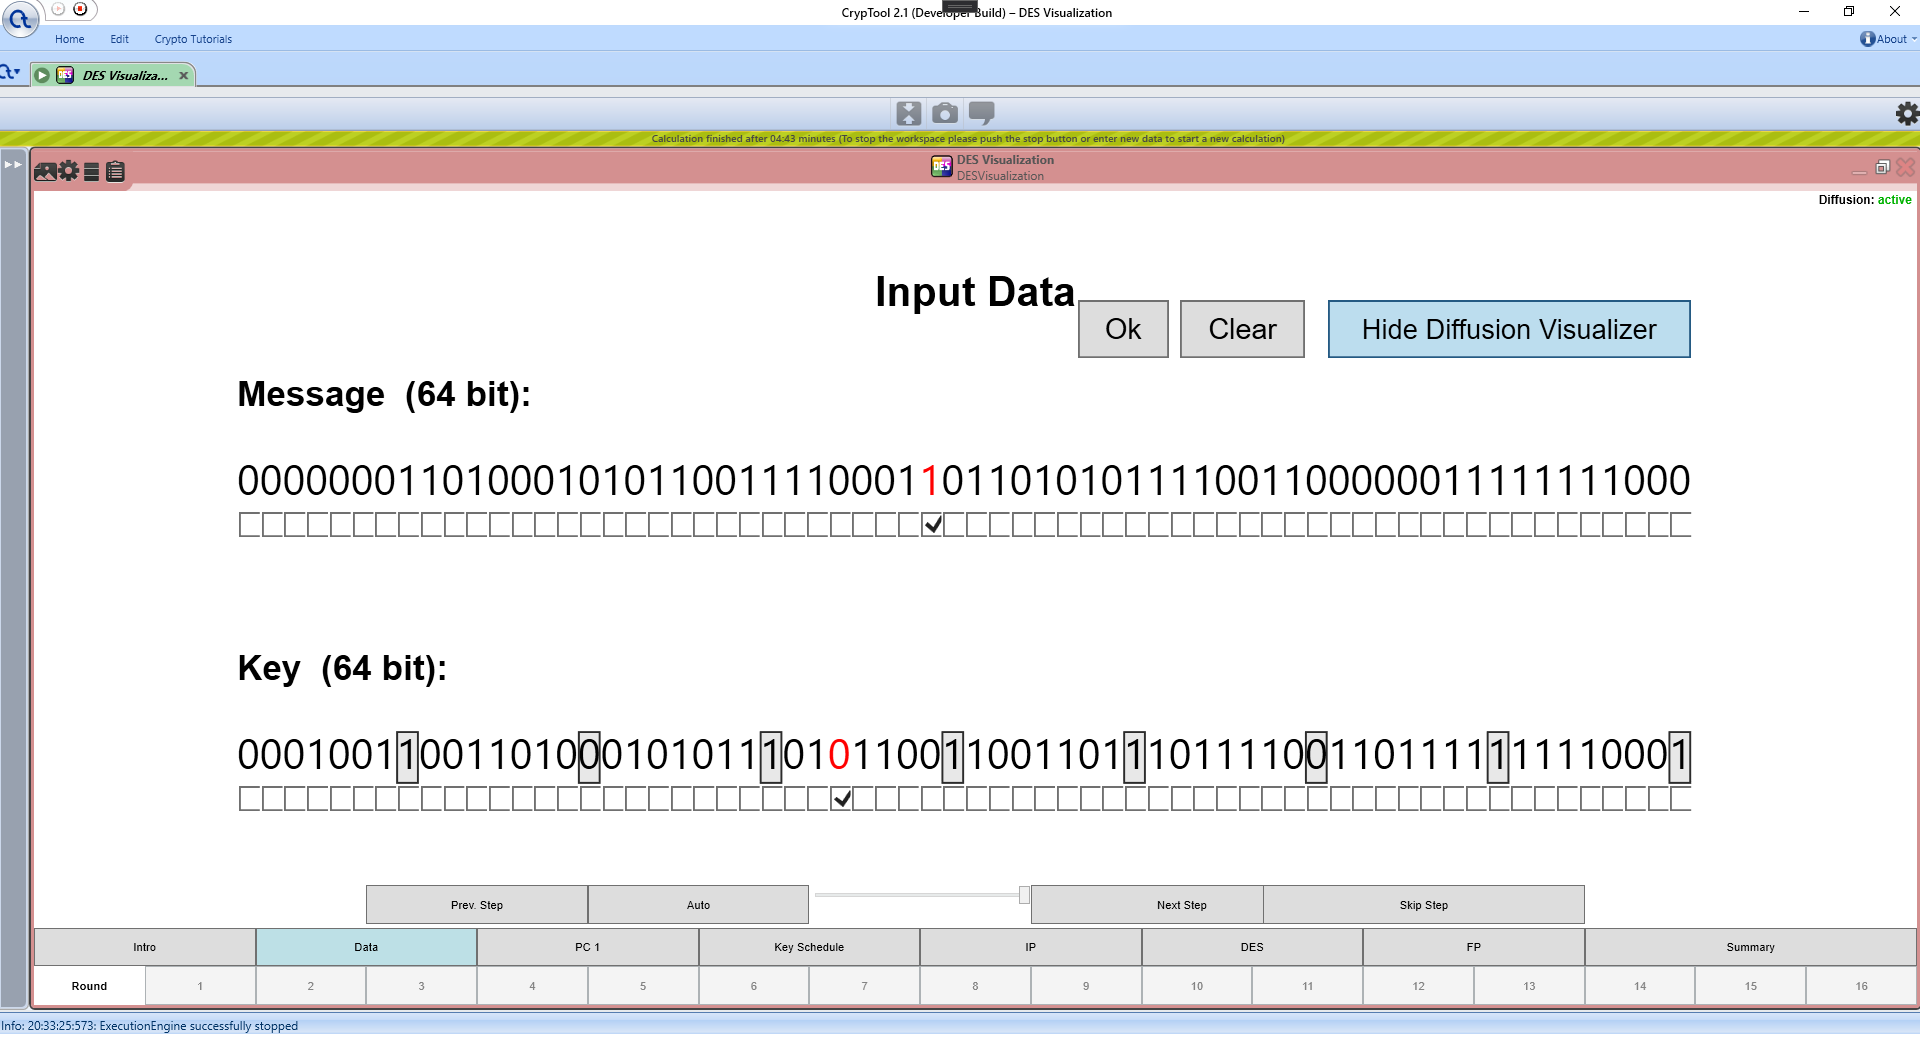
\includegraphics[width=\textwidth]{figures/ct2/des.png}
\caption{DES visualization plug-in}
\label{fig:des}
\end{figure}

The DES visualization was created by Lars Hoffman. His approach to visualizing the diffusion had the most influence on the diffusion visualization in the ChaCha plug-in. In Figure \ref{fig:des}, you can see the page on which the user can flip bits to activate diffusion. The message and key with flipped bits will then be used to show the diffusion property of DES. 

Throughout the visualization, all values are shown in binary. This makes it possible to just mark flipped bits red since if a bit is marked red, we immediately know the value of the diffusion run (we just flip the red bit). 

It was  tried to use the same coloring approach but since the ChaCha cipher uses longer keys and 512-bit blocks compared to the 64-bit blocks of DES, hex strings needed to be used for the values to save canvas space. This lead to a loss of information about the concrete values if only marking red the hexadecimal characters which are different. Therefore, the usage of red color was combined together with showing both values in two rows. In the row for the altered value, the difference is still marked red for easier visual recognition. This is shown later in Figure \ref{fig:chachahash.mid.qr.diffusion}.

\vfill

\pagebreak

\subsection{Avalanche Visualization}
\label{sec:avalancheVisualization}

The Avalanche visualization plug-in was created by Camilo Echeverri in 2016. The most noticeable part about it is probably that it is visually very appealing. Camilo seemed to be very experienced in creating nice user interfaces. Especially the pie chart for the amount of flipped bits with its shadow (Figure \ref{fig:avalanche.roundsend}) and the gradient background stood out. It made it clear that the user interface of the ChaCha visualization should also be visually appealing and not just functional.

The overview over all rounds (Figure \ref{fig:avalanche.overview}) was also a remarkable feature. It was discussed that the ChaCha visualization should include a similar overview since seeing how many rounds were needed for half of all bits to be flipped is useful for studying the diffusion property of a cipher. Unfortunately to date, this did not make it into the version of the plug-in but can be added in the future (see Chapter \ref{sec:futureWork}).

On the other hand, scrollbars as seen in Figure \ref{fig:avalanche.roundsend} should be prevented because the user should see everything he needs immediately.

\begin{figure}
\centering
\begin{subfigure}{\textwidth}
  \centering
  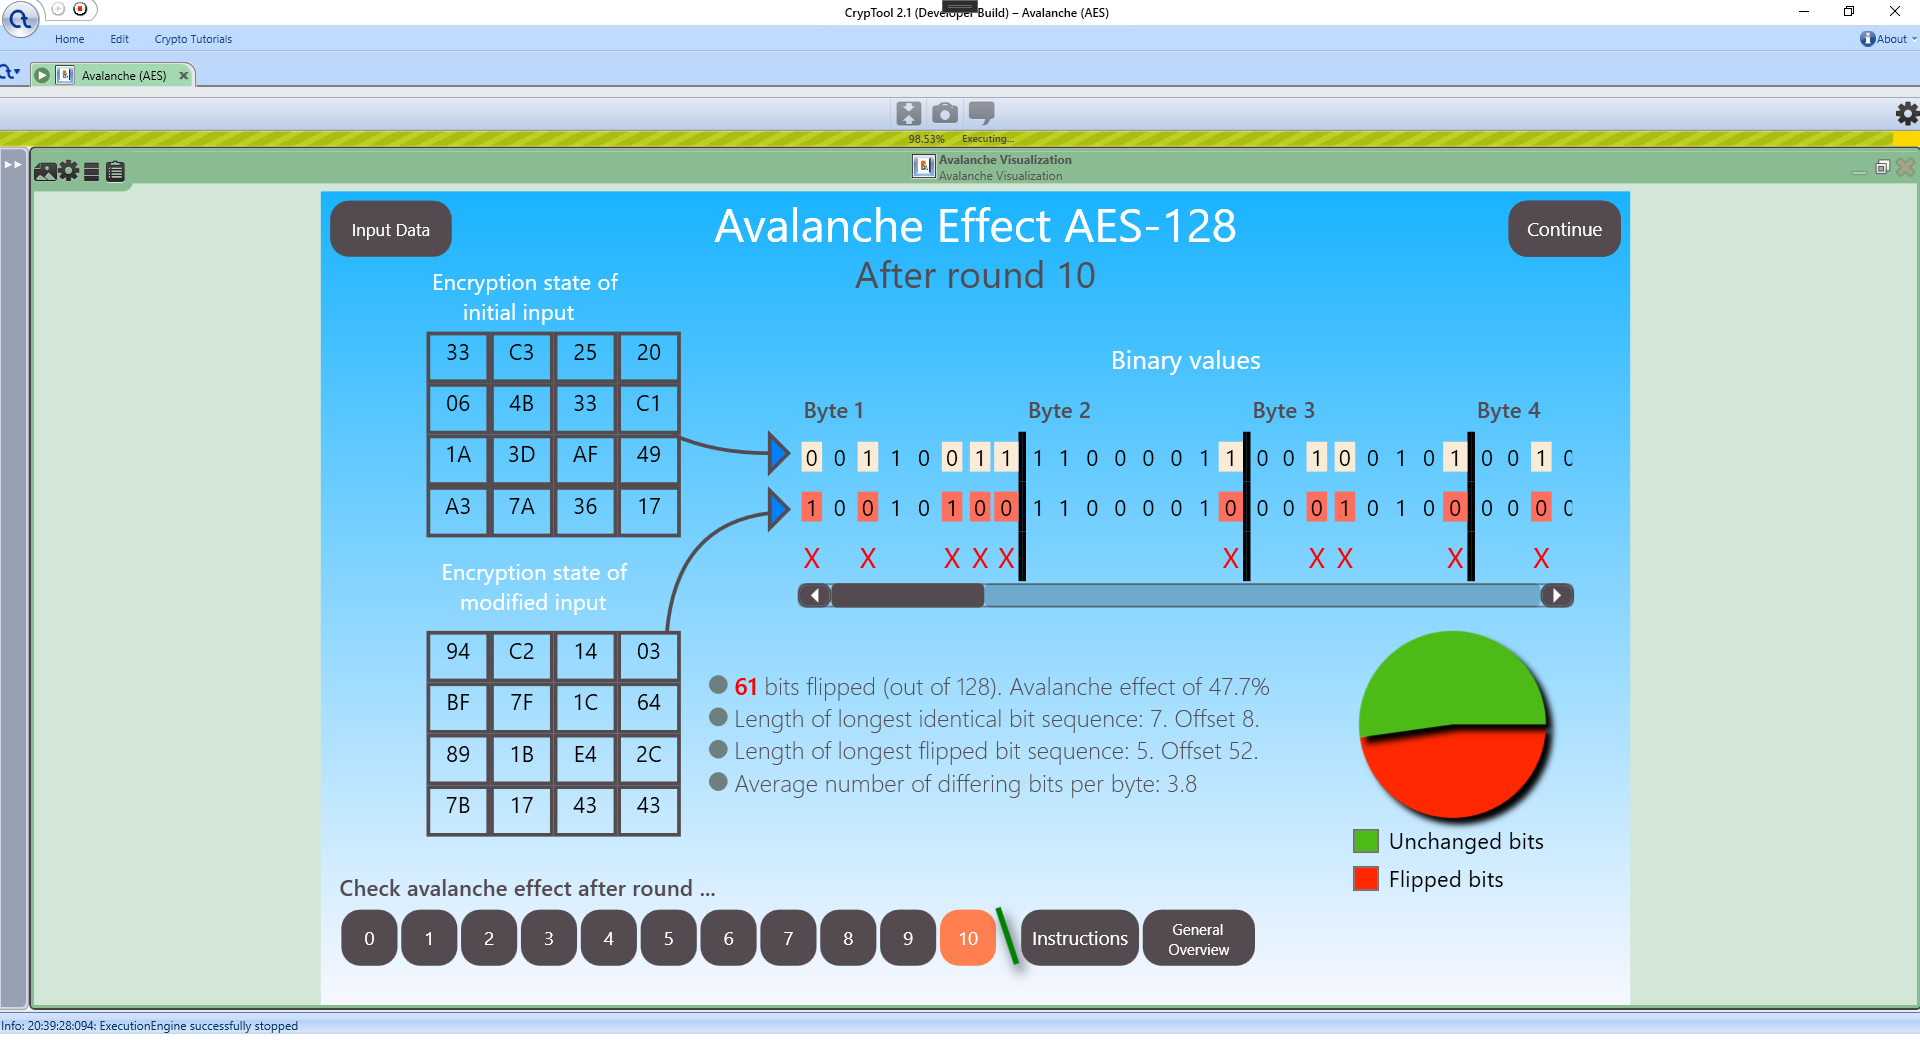
\includegraphics[width=\textwidth]{figures/ct2/avalanche.png}
  \caption{AES-128 avalanche visualization: End of all rounds}
  \label{fig:avalanche.roundsend}
\end{subfigure}
\begin{subfigure}{\textwidth}
  \centering
  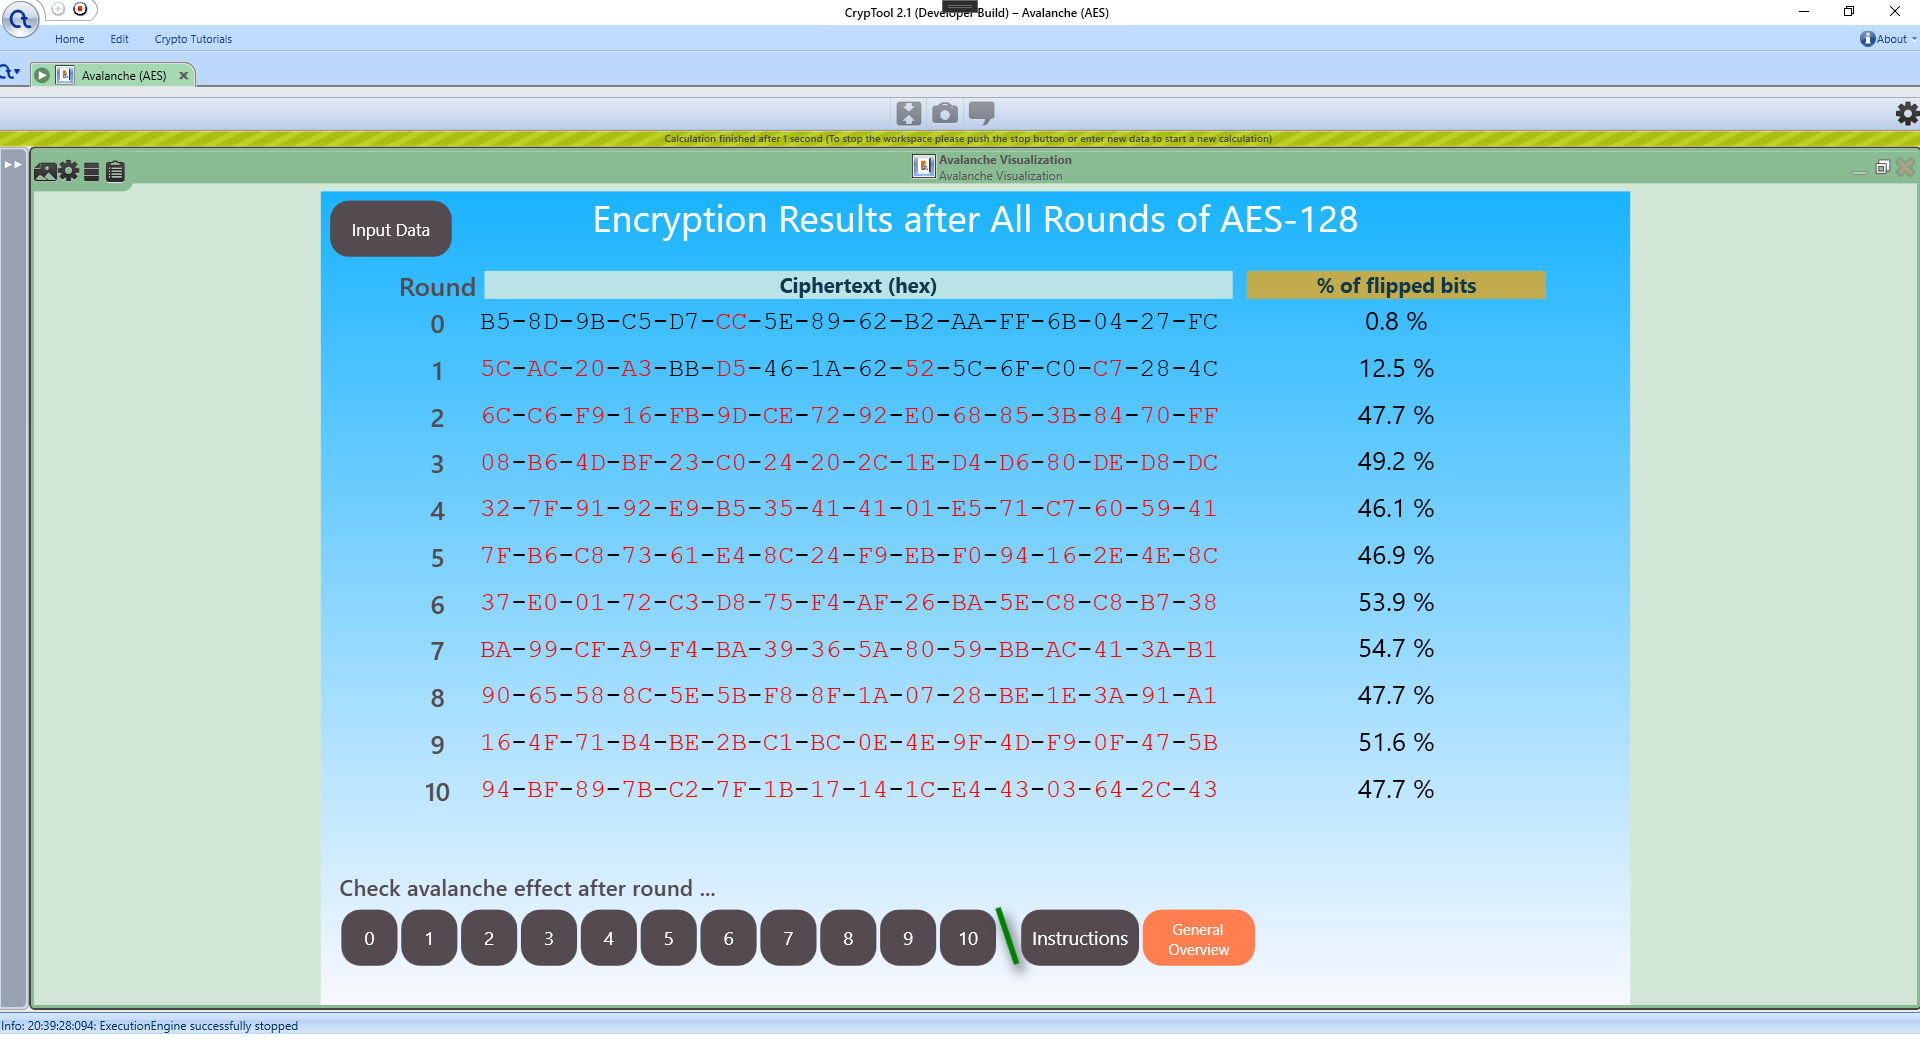
\includegraphics[width=\textwidth]{figures/ct2/avalanche2.png}
  \caption{AES-128 avalanche visualization: General overview}
  \label{fig:avalanche.overview}
\end{subfigure}
\caption{Avalanche visualization plug-in}
\label{fig:avalanche}
\end{figure}
